\documentclass[
	12pt,
	a4paper,
% 	bibtotoc, % obsolet
	bibliography=totoc,
% 	cleardoubleempty, % obsolet
	cleardoublepage=empty,
% 	idxtotoc, % obsolet
	index=totoc,
	ngerman,
	openright
	final,
	listof=nochaptergap,
	hidelinks,
	numbers=noenddot
	]{scrbook}

% ##################################################
% Unterstuetzung fuer die deutsche Sprache
% ##################################################
%\usepackage{ngerman}
\usepackage[ngerman]{babel}
\usepackage[utf8]{inputenc}
%\usepackage{fontspec}
\usepackage{textcomp}
\usepackage{lmodern}

% ##################################################
% Aufzählung mit Prefix \begin{enumerate}[label={Nr. \arabic*}, leftmargin=*, labelindent=1em]
% ##################################################
\usepackage{calc}
\usepackage{enumitem}
\setlist[description]{
  font={\normalfont\itshape\sffamily},
  before={\normalfont\sffamily}
}


% ##################################################
% Dokumentvariablen
% ##################################################

% Persoenliche Daten
\newcommand{\docNachname}{Meiering}
\newcommand{\docVorname}{Helge}
\newcommand{\docStrasse}{Elzstraße 1}
\newcommand{\docOrt}{Winden im Elztal}
\newcommand{\docPlz}{79297}
\newcommand{\docEmail}{h.meiering@hs-furtwangen.de}
\newcommand{\docMatrikelnummer}{256010}

% Dokumentdaten
%\newcommand{\docTitle}{Einsatz von Software Deployment Werkzeugen für OSGi-basierte Gateways am Beispiel von OpenMUC}
%\newcommand{\docTitle}{Evaluation von Open-Source Werkzeugen zur Softwareverteilung für das OSGi-basierte Gateway OpenMUC}
\newcommand{\docTitle}{Konzeption und Implementierung eines Inventarisierungssystem in einer Laborumgebung}
\newcommand{\docUntertitle}{} % Kein Untertitel SW Deploy, IoT, ..., Bingo!
% \newcommand{\docUntertitle}{UNTERTITEL}
% Arten der Arbeit: Bachelorthesis, Masterthesis, Seminararbeit, Diplomarbeit
\newcommand{\docArtDerArbeit}{Masterarbeit}
%Studiengaenge: Allgemeine Informatik Bachelor, Computer Networking Bachelor,
% Software-Produktmanagement Bachelor, Advanced Computer Scinece Master
\newcommand{\docStudiengang}{Mobile Systeme (MOS)}
\newcommand{\docAbgabedatum}{\today}
\newcommand{\docErsterReferent}{Prof. Dr. Elmar Cochlovius}
\newcommand{\docZweiterReferent}{Judith Jakob} % Wenn es nur einen Betreuer gibt
% \newcommand{\docZweiterReferent}{-}

% ##################################################
% Allgemeine Pakete
% ##################################################

% Abbildungen einbinden
\usepackage{graphicx}
\usepackage{float}
\usepackage{framed}

% Farben
\usepackage{color}
\usepackage[usenames,dvipsnames,svgnames,table]{xcolor}

% Maskierung von URLs und Dateipfaden
\usepackage[hyphens,spaces,obeyspaces]{url}

% setzt Tabellen auch dorthin, wo sie erstellt wereden!
\usepackage[section]{placeins}
% Deutsche Anfuehrungszeichen
\usepackage[babel, german=quotes]{csquotes}

% Pakte zur Index-Erstellung (Schlagwortverzeichnis)
% \usepackage{index}
% \makeindex

% Ipsum Lorem
% Paket wird nur für das Beispiel gebraucht und kann gelöscht werden
\usepackage{lipsum}

% ##################################################
% Seitenformatierung
% ##################################################
\usepackage[
	portrait,
	bindingoffset=1.5cm,
	inner=2.5cm,
	outer=2.5cm,
	top=3cm,
	bottom=2cm,
	%showframe,
	%includeheadfoot
	]{geometry}

% ##################################################
% Kopf- und Fusszeile
% ##################################################





%\renewcommand\chaptermarkformat{\ifnumbered{chapter}{\chapapp\ \thechapter. \ }{}}


\usepackage{fancyhdr}

\pagestyle{fancy}
\fancyhf{}
\fancyhead[EL,OR]{\sffamily\thepage}
\fancyhead[ER,OL]{\sffamily\leftmark}
%\fancyhead[EL,OR]{\sffamily\bfseries\thepage}
%\fancyhead[ER,OL]{\sffamily\bfseries\leftmark}

\fancypagestyle{headings}{}
\fancypagestyle{plain}{}

%\fancypagestyle{empty}{
%  \fancyhf{}
%  \renewcommand{\headrulewidth}{0pt}
%}

%Kein "Kapitel # NAME" in der Kopfzeile
%\renewcommand{\chaptermark}[1]{
%	\markboth{#1}{}
%  	\markboth{\thechapter.\ #1}{}
%}

% ##################################################
% Schriften
% ##################################################

% Stdandardschrift festlegen
\renewcommand{\familydefault}{\sfdefault}

% Standard Zeilenabstand: 1,5 zeilig
\usepackage{setspace}
%\onehalfspacing 

% Schriftgroessen festlegen
\addtokomafont{chapter}{\sffamily\large\bfseries} 
\addtokomafont{section}{\sffamily\normalsize\bfseries} 
\addtokomafont{subsection}{\sffamily\normalsize\mdseries} 
\addtokomafont{caption}{\sffamily\normalsize\mdseries} 
% \addtokomafont{paragraph}{\sffamily\normalsize\mdseries}

% ##################################################
% Inhaltsverzeichnis / Allgemeine Verzeichniseinstellungen
% ##################################################

\usepackage{tocloft}

% Punkte auch bei Kapiteln
\renewcommand{\cftchapdotsep}{3}
\renewcommand{\cftdotsep}{3}

% Schriftart und -groesse im Inhaltsverzeichnis anpassen
\renewcommand{\cftchapfont}{\sffamily\normalsize}
\renewcommand{\cftsecfont}{\sffamily\normalsize}
\renewcommand{\cftsubsecfont}{\sffamily\normalsize}
\renewcommand{\cftchappagefont}{\sffamily\normalsize}
\renewcommand{\cftsecpagefont}{\sffamily\normalsize}
\renewcommand{\cftsubsecpagefont}{\sffamily\normalsize}

%Zeilenabstand in den Verzeichnissen einstellen
\setlength{\cftparskip}{.5\baselineskip}
\setlength{\cftbeforechapskip}{.1\baselineskip}

% ##################################################
% Abbildungsverzeichnis und Abbildungen
% ##################################################

\usepackage{caption}

\usepackage{wrapfig}
\usepackage{framed}

% Nummerierung von Abbildungen
\renewcommand{\thefigure}{\arabic{figure}}
\usepackage{chngcntr}
\counterwithout{figure}{chapter}

% Abbildungsverzeichnis anpassen
\renewcommand{\cftfigpresnum}{Abbildung }
\renewcommand{\cftfigaftersnum}{:}

% Breite des Nummerierungsbereiches [Abbildung 1:]
\newlength{\figureLength}
\settowidth{\figureLength}{\bfseries\cftfigpresnum\cftfigaftersnum}
%\setlength{\cftfignumwidth}{\figureLength}
\setlength{\cftfignumwidth}{2.6cm}
\setlength{\cftfigindent}{0cm}

% Schriftart anpassen
\renewcommand\cftfigfont{\sffamily}
\renewcommand\cftfigpagefont{\sffamily}

\usepackage{subcaption}

% ##################################################
% Tabellenverzeichnis und Tabellen
% ##################################################

% Nummerierung von Tabellen
\renewcommand{\thetable}{\arabic{table}}
\counterwithout{table}{chapter}
\usepackage{tabu}
\usepackage{booktabs}

% Fußnoten in Tabellen
\usepackage{threeparttable} 
\usepackage{multirow}

\usepackage[table]{xcolor}
\usepackage{etoolbox}
\AtBeginEnvironment{tabular}{\footnotesize}
\AtBeginEnvironment{longtable}{\footnotesize}

% Dadurch können mit x{size} rechtsbündige und mit z{size} zentrierte Zellen
% mit fester Größe size erstellt werden.
\newcolumntype{y}[1]{>{\raggedright\arraybackslash\hspace{0pt}}p{#1}}
\newcolumntype{x}[1]{>{\raggedleft\arraybackslash\hspace{0pt}}p{#1}}
\newcolumntype{z}[1]{>{\centering\arraybackslash\hspace{0pt}}p{#1}}

% Tabellenverzeichnis anpassen
\renewcommand{\cfttabpresnum}{Tabelle }
\renewcommand{\cfttabaftersnum}{:}

% Breite des Nummerierungsbereiches [Abbildung 1:]
\newlength{\tableLength}
\settowidth{\tableLength}{\bfseries\cfttabpresnum\cfttabaftersnum}
%\setlength{\cfttabnumwidth}{\tableLength}
\setlength{\cfttabnumwidth}{2.0cm}
\setlength{\cfttabindent}{0cm}

%Schriftart anpassen
\renewcommand\cfttabfont{\sffamily}
\renewcommand\cfttabpagefont{\sffamily}

% Unterdrueckung von vertikalen Linien
\usepackage{booktabs}

% ##################################################
% Listings (Quellcode)
% ##################################################

\usepackage{listings}
\definecolor{gray}{rgb}{0.4,0.4,0.4}
\definecolor{darkblue}{rgb}{0.0,0.0,0.6}
\definecolor{cyan}{rgb}{0.0,0.6,0.6}

\lstset{
  basicstyle=\ttfamily,
  %basicstyle=\normalsize,
  columns=fullflexible,
  showstringspaces=false,
  breaklines=true,
  breakautoindent=true,
  numbers=left,
  numberstyle=\tiny,
  numbersep=5pt,
  keywordstyle=\color{blue},
  commentstyle=\color{green},   
  stringstyle=\color{gray},
  linewidth=14.6cm,
  xleftmargin=0.45cm,
}

\lstdefinelanguage{XML}
{
  morestring=[b]",
  morestring=[s]{>}{<},
  morecomment=[s]{<?}{?>},
  stringstyle=\color{black},
  identifierstyle=\color{darkblue},
  keywordstyle=\color{cyan},
  morekeywords={xmlns,version,type}% list your attributes here
}

% \lstset{
% 	language=java,
% 	backgroundcolor=\color{white},
% 	breaklines=true,
% 	prebreak={\carriagereturn},
%  	breakautoindent=true,
%  	numbers=left,
%  	numberstyle=\tiny,
%  	stepnumber=2,
%  	numbersep=5pt,
%  	keywordstyle=\color{blue},
%    	commentstyle=\color{green},   
%    	stringstyle=\color{gray}
% }
  	
% ##################################################
% Theoreme
% ##################################################
  	
% Umgebung fuer Beispiele
\newtheorem{beispiel}{Beispiel}

% Umgebung fuer These
\newtheorem{these}{These}

% Umgebung fuer Definitionen
\newtheorem{definition}{Definition}
  	
% ##################################################
% Literaturverzeichnis
% ##################################################

\usepackage{bibgerm}
%\usepackage{apacite}
\usepackage[backend=biber, bibencoding=utf8, style=alphabetic,]{biblatex}
%\bibliography{bibitems}
\addbibresource{literatur.bib}


% ##################################################
% Abkuerzungsverzeichnis
% ##################################################

%\usepackage[printonlyused]{acronym}
\usepackage{acronym}
%\renewcommand*{\acsfont}[1]{\normalfont\bfseries #1}

% ##################################################
% PDF / Dokumenteninternelinks
% ##################################################

\usepackage[
    unicode=true,
    pdfencoding=unicode,
    colorlinks=false,
    linkcolor=black,
    citecolor=black,
    filecolor=black,
    urlcolor=black,
    bookmarks=true,
    bookmarksopen=true,
    bookmarksopenlevel=3,
    bookmarksnumbered,
    plainpages=false,
    pdfpagelabels=true,
    hyperfootnotes,
    subfigure,
    pdftitle ={\docTitle},
    pdfauthor={\docVorname~\docNachname},
    pdfcreator={\docVorname~\docNachname}]{hyperref}

\usepackage[all]{nowidow}

\makeindex
 
\begin{document}


% \nocite{ploetner}
 \nocite{windows}
\setcounter{secnumdepth}{3}
\setlength{\parindent}{0pt} % mach das Einrücken weg bei neuen Abschnitten
% Titelblatt
\begin{titlepage}
\pagestyle{empty}

% ##################################################
% HFU-Logo einbinden
% ##################################################
\begin{flushright}
\begin{figure}[ht]
\flushright

\includegraphics[height=3cm]{content/pictures/hfu.jpg}
\end{figure}
\end{flushright}

% ##################################################
% Titel
% ##################################################
\begin{center}
{\fontsize{18}{22} \selectfont \docArtDerArbeit}\\[5mm]
{\fontsize{18}{22} \selectfont im Studiengang} \\[5mm]
{\fontsize{18}{22} \selectfont \docStudiengang}\\
\vspace{1cm}
\begin{onehalfspace}
{\fontsize{22}{26} \selectfont \textbf{\docTitle}}\\[5mm]
% {\fontsize{18}{22} \selectfont \docUntertitle}


\end{onehalfspace}
\end{center}

% ##################################################
% Zusatzinformationen
% ##################################################
\vfill
\begin{center}
\begin{tabular}{lcl}
Referent  		&:& \docErsterReferent 	\\ \\
Koreferent 		&:& \docZweiterReferent \\ \\	
Vorgelegt am 	&:& \docAbgabedatum 	\\ \\
Vorgelegt von 	&:& \docVorname~\docNachname\\
				& & Matrikelnummer: \docMatrikelnummer\\
				& & \docStrasse,~\docPlz~\docOrt	\\
				& & \docEmail			
\end{tabular}
\end{center}
\end{titlepage}
\cleardoubleemptypage

\frontmatter % römische Seitennummerierung

\onehalfspacing 
% Abstract
\chapter*{Abstract\markboth{Abstract}{}}
\addcontentsline{toc}{chapter}{Abstract}

The present work shows how an inventory system can look like in a laboratory environment. A lot of importance is attached to the conception. In this phase, it is not only decided how the application should look at the end, but also how it is implemented. The knowledge of the developer has to be considered. It is necessary to measure the amount of learning required to familiarize yourself with the new and unknown technologies. At the end, an implementation must take place, which presents many challenges.


Die vorliegende Arbeit zeigt wie sich ein Inventarsystem in einer Laborumgebung aussehen kann. Dabei wird ein großer Wert auf die Konzeption gelegt. In dieser Phase entscheidet sich nicht nur wie die Anwendung zum Schluss aussehen soll, sondern auch wie sie umgesetzt wird. Es muss das Wissen vom Entwickler berücksichtigt werden. Dabei muss der Lernaufwand bemessen werden, welcher benötigt wird um sich in die neuen, noch unbekannten Technologien einzuarbeiten. Zum Schluss muss eine Umsetzung erfolgen, welche viele Herausforderungen stellt.

\cleardoubleemptypage
\singlespacing
% Inhaltsverzeichnis
\phantomsection
\tableofcontents
\addcontentsline{toc}{chapter}{Inhaltsverzeichnis}
\cleardoubleemptypage

% Abbildungsverzeichnis einbinden und ins Inhaltsverzeichnis
% WORKAROUND: tocloft und KOMA funktionieren zusammen nicht
% korrekt\phantomsection
\phantomsection
\addcontentsline{toc}{chapter}{\listfigurename} 
\listoffigures
\cleardoubleemptypage

% Tabellenverzeichnis einbinden und ins Inhaltsverzeichnis
% WORKAROUND: tocloft und KOMA funktionieren zusammen nicht
% korrekt\phantomsection
%\phantomsection
%\addcontentsline{toc}{chapter}{\listtablename}
%\listoftables
%\cleardoubleemptypage

% Abkürzungsverzeichnis
\chapter*{Abkürzungsverzeichnis\markboth{Abkürzungsverzeichnis}{}}
\addcontentsline{toc}{chapter}{Abkürzungsverzeichnis}

\begin{acronym}
	\acro{bzw.}{beziehungsweise}
	\acro{CD}{Corporate Design}
	\acro{CLI}{Command Line Interface}
	\acro{CMS}{Content Management System}
	\acro{CORS}{Cross-Origin Resource Sharing}
	\acro{CSS}{Cascading Style Sheets}
	\acro{Ecma}{Ecma International}
	\acro{FTP}{File Transfere Protocol}
	
	\acro{GNU}{General Public License}
	\acro{GPL}{General Public License}
	
	\acro{HTML}{Hypertext Markup Language}
	 \acro{HTTP}{Hypertext Transfer Protocol}
	
	\acro{IDE}{integrated development environment}
	\acro{IP}{Internet Protocoll Adresse}
	
	\acro{JSON}{JavaScript Object Notation}
	
	\acro{MAC}{Media-Access-Control-Adresse}
	\acro{MIT}{Massachusetts Institute of Technology}
	
	\acro{MVC}{Modell View Controller}
	\acro{NPM}{Node Package Manager}
	\acro{REST}{Representational-State-Transfer}
	
	
	\acro{UI}{User-Interface}
	\acro{uvm.}{und vieles mehr}
	
	\acro{URL}{Uniform Resource Locator}
	\acro{UX}{User Experience}


	\acro{WLAN}{Wireless-Local-Area-Network}
	
	\acro{PDO}{PHP: Data Objects}
	\acro{PHP}{PHP: Hypertext Preprocessor}

	\acro{SASS}{Syntactically Awesome Stylesheets}
	\acro{SCP}{Secure Copy}
	\acro{SHL}{Smart Home Labor}
	
	\acro{SSH}{Secure Shell}
	\acro{SOP}{Same-Origin-Policy}
	\acro{SQL}{Structured Query Language}



	
	\acro{VM}{Virtuelle Maschine}
	
	\acro{XML}{Extensible Markup Language}
	\acro{z. Dt.}{zu Detusch}

\end{acronym}


\mainmatter % arabische Seitennummerierung
\onehalfspacing 
\chapter{Einleitung}
Das Smarthome-Labor der Hochschule Furtwangen umfasst vier einzelne Räume und ein Arbeitsbereich, in welchem sich Studierende, Mitarbeiterinnen und Mitarbeiter sich auf ihre wichtigen Arbeiten im Labor konzentrieren können. Das noch junge Labor steckt voller Leben. Es wird mit Bachelor-Projekten, Bachelor-Thesen und Master-Thesen immer weiter ausgebaut und die Studierenden lernen praxisnah den Umgang mit Geräten in einer Smarthome-Umgebung. Diese betrifft nicht nur die Unterkunft in welcher Personen leben, sondern auch die Industrie 4.0.

Im Sommersemester 2017 entstand die Masterthesis von Ashiq Mohamed Akbar Ali mit dem Titel "Creating a website with Info-Terminal and Live CCTV Stream for the Smart Home Laboratory at the Hochschule Furtwangen University". Mit dieser Arbeite wurde das Labor mit einer umfangreichen Webpräsenz ausgestattet, welche einen Einblick über die die Vielfalt im Labor gibt. Das Labor wird hierbei vorgestellt und es wird auf einzelne Details eingegangen.

Es gibt eine Vielzahl an Geräten, Sensoren, Mikrocomputer und Alltagsgegenstände, wie zum Beispiel das Bett, mit welchen die Studierenden experimentieren und einen Betrag für die Wissenschaft und Öffentlichkeit bieten können.


\autocite{JustinEllingwood.2016b}

\section{Problemstellung}
\label{sec:Problemstellung}

Durch diese große Anzahl von Geräten, Sensoren und Mikrocomputer entsteht auch eine Unübersichtlichkeit. Zwar wurden alle Gegenstände erfasst und Dokumentiert, jedoch ist das nur in einer Tabelle erfasst worden. Ein Durchsuchen dieser Tabelle kann Aufwendig sein wenn ein bestimmtes Gerät und dessen Status überprüft werden soll. Für ihre Arbeiten müssen sich Studenten auch Geräte reservieren oder gar ausleihen um sie in fremden Umgebungen testen zu können oder um daheim weiter arbeiten zu können. Dies in einer Tabelle zu erfassen ist nicht unmöglich, aber es handelt sich hierbei um einen großen Aufwand. Dieser gestaltet die Arbeit von einer Mitarbeiterin oder einem Mitarbeite, als sehr Aufwendig. Diese Tabelle muss ständig kontrolliert und aktualisiert werden. Auch muss geprüft werden, ob die Leihe für ein Gerät schon verstrichen ist.


\section{Ziel der Arbeit}
\label{sec:ziel}
Ziel ist eine Übersicht in das Umfangreiche Inventar des Smarthome-Labors zu geben. Dabei kann eine Webanwendung helfen, welche in einer Tabelle Alle Geräte, Sensoren und Mikrocomputer Aufnimmt. Diese Tabelle kann mittels Software schnell durchsucht und einfach erweitert werden. Auch soll die Mitarbeiterin oder der Mitarbeiter, wie auch Studierende an das Ende einer Leihfrist erinnert werden. Auch hierbei ist die Software eine Lösung, indem sie Erinnerungsmails verschickt.


\chapter{Vorgehen}
In der Vorbereitung wurden schon früh die Werkzeuge für die Umsetzung und Konzeption gewählt, welche das Projekt strukturieren und planen sollten. Dabei kamen Mittel wie Kugelschreiber, Notizbücher, Kalender oder auch die Mindmap zum Einsatz. Mittels Requirement Engeneering wurde eine Anforderungsanalyse erstellt. Um einen übersichtlichen Workflow zu haben, fiel die Entscheidung Scrum als Vorgehensmodell für den künftigen Ablauf zu wählen.

\section{Versionsverwaltung}
Für die Versionsverwaltung wurde Git gewählt. Es handelt sich um ein Dezentrales Versionsverwaltungssystem und ist nicht von einem Bestimmten Server verbunden. In einem Versionsverwaltungssystem werden Verschiedene Entwicklungszustände gesichert. Damit ist es möglich zu sehen, wie sich eine Software entwickelt hat. Sollte ein Fehler auftreten, kann zu einer älteren Version gewechselt werden, in welcher der Fehler nicht vorhanden ist. Diese Versionen werden in einem Repository verwaltet.\autocite{git}



\section{Scrum}
\label{scrum}

Unter Scrum versteht man in der Projektplanung ein agiles Vorgehensmodell in der Softwareentwicklung. Es besteht aus mehreren Komponenten wie, Rollen Artefakte und Meetings. Sobald die Anforderungen und Eigenschaften eines Produktes angelegt worden sind, legt sie der Product Owner in einem sogenannten Product Backlog an. Daraufhin wird ein Sprint geplant. Es werden Anforderungen und Eigenschaften gewählt, welche in einem bestimmten Zeitraum erledigt werden können. Diese wiederum werden in das sogenannte Sprint Backlog abgelegt. Darauf erfolgt ein Sprint. Welcher nicht länger al ein Monat dauern sollte. Während des Sprints Tauscht sich das Entwicklerteam über den täglichen Status der Entwicklung aus. Man spricht von einem Daily Meeting. Jeder ist auf dem aktuellen Stand und es kann sofort eingegriffen werden, wenn es an einer Stelle zu Schwierigkeiten kommt. Ist ein Sprint abgeschlossen kann ein funktionierender Softwareteil präsentiert werden. \autocite{Niermann.2017}

\begin{figure}[H]
	\centering
	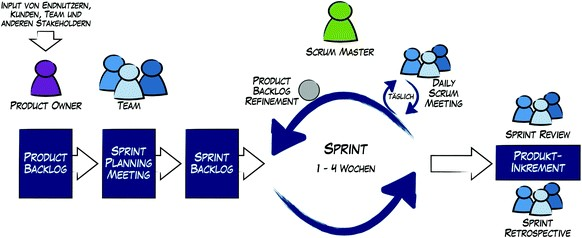
\includegraphics[scale=0.95]{content/pictures/scrum.jpg}
	% bosch_iot_poll.png: 0x0 pixel, 300dpi, 0.00x0.00 cm, bb=
	\caption{Ablauf eines Scrums. \cite{Niermann.2017}}
	\label{fig:scrum}
\end{figure}

\subsection{Scrum als Einzelperson}
In dieser Arbeit wurde alleine und nicht im Team gearbeitet. Auch wenn es hierdurch keine Rollenverteilung gab, so konnte Scrum doch ideal eingesetzt werden. Das Backlog wurde mit Hilfe der Konzeption erzeugt. Mit der Planung wurde klar, welche Anforderungen an die Software bestehen. Diese wurden alle handschriftlich in ein Productbacklog niedergeschrieben. Darauf wurde mit dem Betreuer besprochen, welche aufgaben innerhalb von zwei Wochen erledigt seien sollen und wurden, ebenfalls handschriftlich, in das Sprintbacklog aufgenommen. Während des Sprints sind die Daily Meetings entfallen, da diese nicht nötig waren. Als einzelne Person ist man immer über den aktuellen Stand seiner Entwicklung bewusst. Ein tägliches Austauschen mit Teammitglieder ist nicht nötig, da es kein Team gibt. Nach den vergangenen zwei Wochen, wurde der Aktuelle Stand in einem Protokoll dokumentiert. Erfolge und Probleme wurden im Anschluss mit dem Erstbetreuer und der Zweitbetreuerin besprochen. Daraufhin wurde, wenn es nötig wurde, das Productbacklog erweitert. Aus diesem  Backlog wurden erneut Aufgaben für den nächsten Sprint gewählt. Der Entwickler übernahm so alle Rollen, welche in dem Vorgehensmodell Scrum definiert sind.


\chapter{Konzeption}
\label{cha:konzeption}
Bei der Konzeption wurde der aktuelle Stand des bestehenden Webauftritts betrachtet und analysiert. Im weiteren Schritt wurden Erweiterungen für die Website geplant. Im nächsten großen Schritt erfolgte eine Analyse aktuell bestehender Software, welche Gegenstände verwaltet.


\section{Analyse des aktuellen Webauftritts}
\label{webauftritt}
Der Webauftritt, erreichbar im Netzwerk der Hochschule Furtwangen\url{http://web.smarthome.hs-furtwangen.de/}, des \ac{SHL} Labors, wird mit der Hilfe des \ac{CMS} WordPress verwaltet. WordPress eigne sich hier, weil es mittels \ac{UX} so gestaltet wurde, das es sehr leicht zu erlernen ist. Unerfahrene Benutzer könne so schnell eigene Inhalte einpflegen.

\begin{figure}[bh]
	\centering
	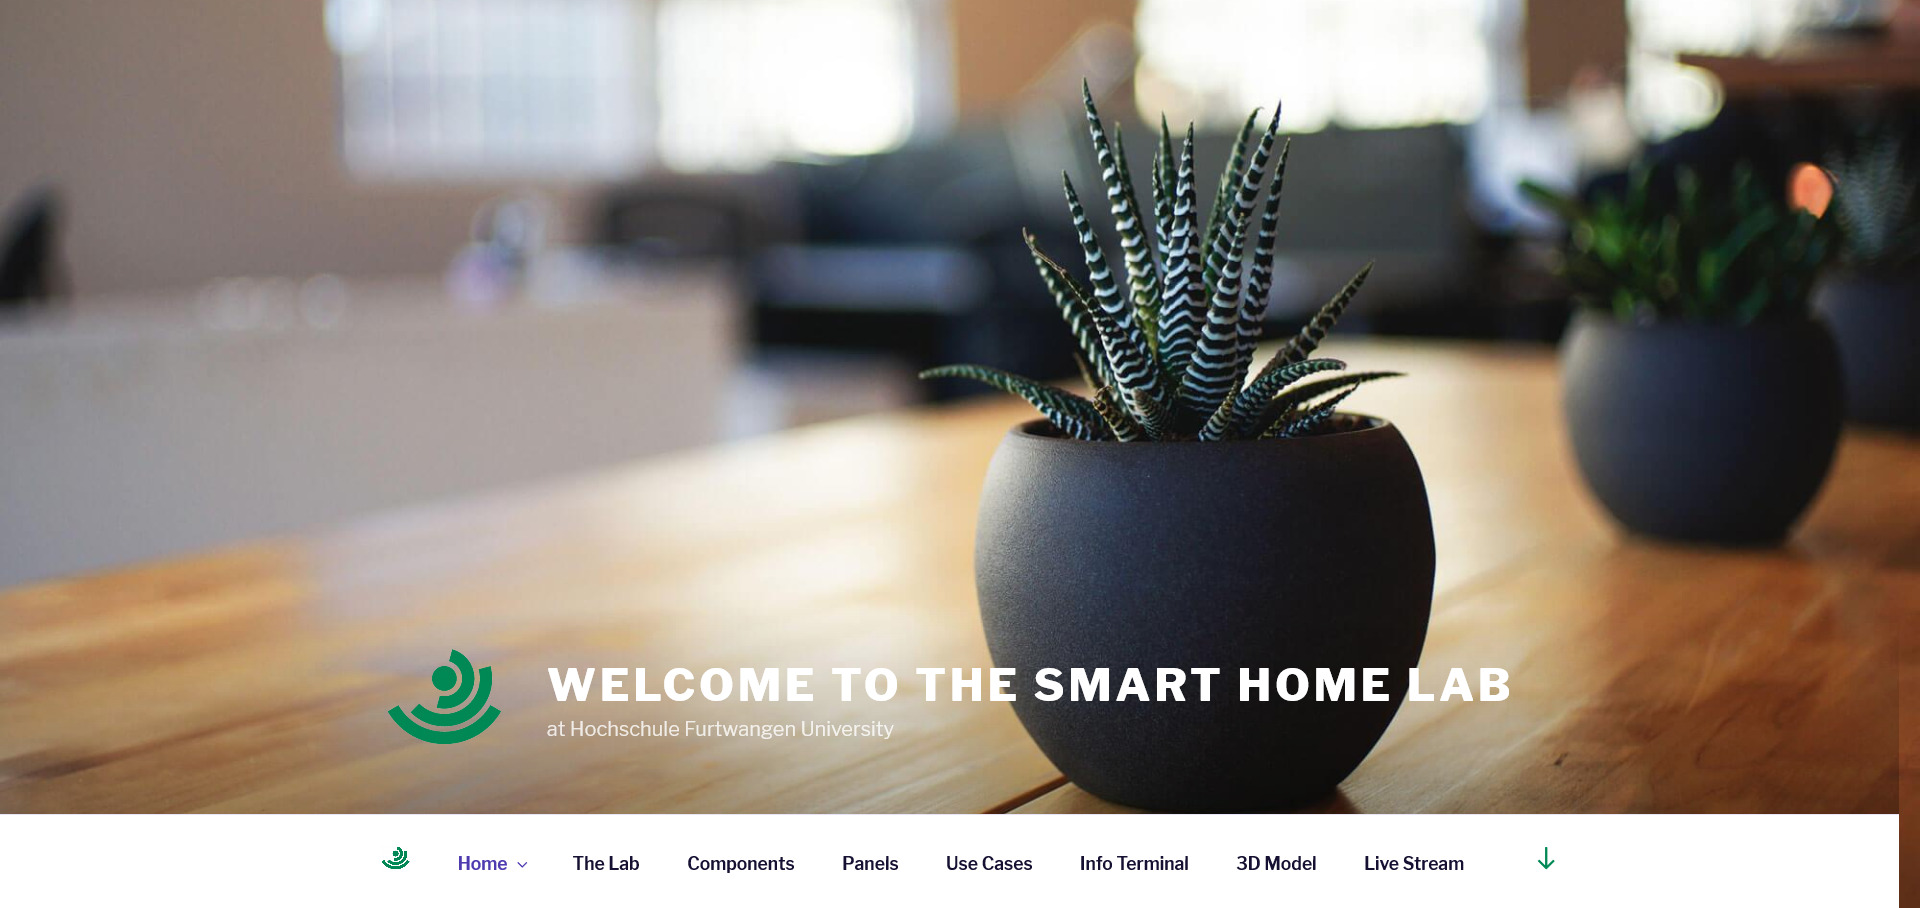
\includegraphics[scale=0.23]{content/pictures/shlwebsit.jpg}
	% bosch_iot_poll.png: 0x0 pixel, 300dpi, 0.00x0.00 cm, bb=
	\caption{Die Startseite des Webauftritts}
	\label{fig:web}
\end{figure}

Die Website ist mit dem, von WordPress eigenem Designe Twentyseventeen gestaltet. Auf der Startseite sieh man ein großes Headerbild. Darunter Folgt eine Navigationsleiste, welche die Links bei einem Besuch einer Unterseite in einem Lila Farbton darstellt. Die Navigation umfasst die Seiten:

\begin{itemize}
	\item Home
	
	\item The Lab 
	
	\item Components 
	
	\item Panels
	
	\item Use Cases 
	
	\item Info Terminal
	
	\item 3D Model
	
	\item Live Stream
	
	
	
\end{itemize}

Weiter folgt eine kurze Beschreibung über das Labor. Der nächste Abschnitt der Startseite stellt das Team vor. Im Anschluss sieht man noch ein Video, welches das Labor vorstellt, ein Kontaktforumlar und die Addresse mit einer Google Maps Karte. Am untersten Ende ist ein Footer, welche eine Copyright und einen Link zum Impressum enthält.

Die Unterseite \glqq The Lab\grqq stellt das Labor mit Grundrissen etwas detailreicher vor. \glqq Components\grqq stellt wenige, aber wichtige Geräte vor. In \glqq Panels\grqq werden, die mit Sensoren und Geräte versehenen, Wände in den Räumen beschrieben. Eine Auswahl von umgesetzten Anwendungsfällen werden in der Unterseite \glqq Use Cases\grqq beschrieben. Für das Infoterminal gibt es ebenfalls eine Unterseite, welche automatisiert eine Präsentation über das Labor abspielt. Unter dem Punkt \glqq 3D Model\grqq, befindet sich eine 3D Ansicht des Labors, welches sich in einer Ego- und Vogelperspektive betrachten lässt. Auch können hier vereinzelt Geräte bedient werden. Abgeschlossen wird die Navigation mit einer Unterseite, welche einen Video Livestream zeigen kann.

 

\subsection{Corporate Design}
Mit den aktuellen Farben entspricht der Webauftritt des Labors nicht dem \ac{CD} der Hochschule Furtwangen. So müssen die Lila Farben durch die Farbe Grün mit dem Hexwert 83b62d geändert werden. Dies ist wichtig um einen Wiedererkennungswert der Hochschule darzustellen. Die Navigation stellte hier einen größeren Bruch dar. Um die Seite vollständig im \ac{CD} der Hochschule zu haben, ist ein Expertengespräch nötig.



\subsection{Erweiterung des Webauftritts}
Neben dem \acf{CD} gab es noch weitere Punkte, welche den Auftritt noch Informativer und attraktiver gestalten konnten. So stehen im Labor die einzelnen Räume: Küche, Bad, Multimediaraum, IoT-Raum und der Arbeitsbereich stark im Vordergrund. Diese wurden bisher nur sehr dürftig auf der Homepage erwähnt. Daher wurde für die Räume eigene Unterseiten angelegt. Um auf \acf{UX} zu achten, wurde mittels des WordPress-Plugin Draw Attention  eine Interaktive Karte erzeugt. Bei einem Klick auf einen Raum, erhält der User mehr Informationen. \autocite{WPDrawAttention.}

\begin{figure}[H]
	\centering
	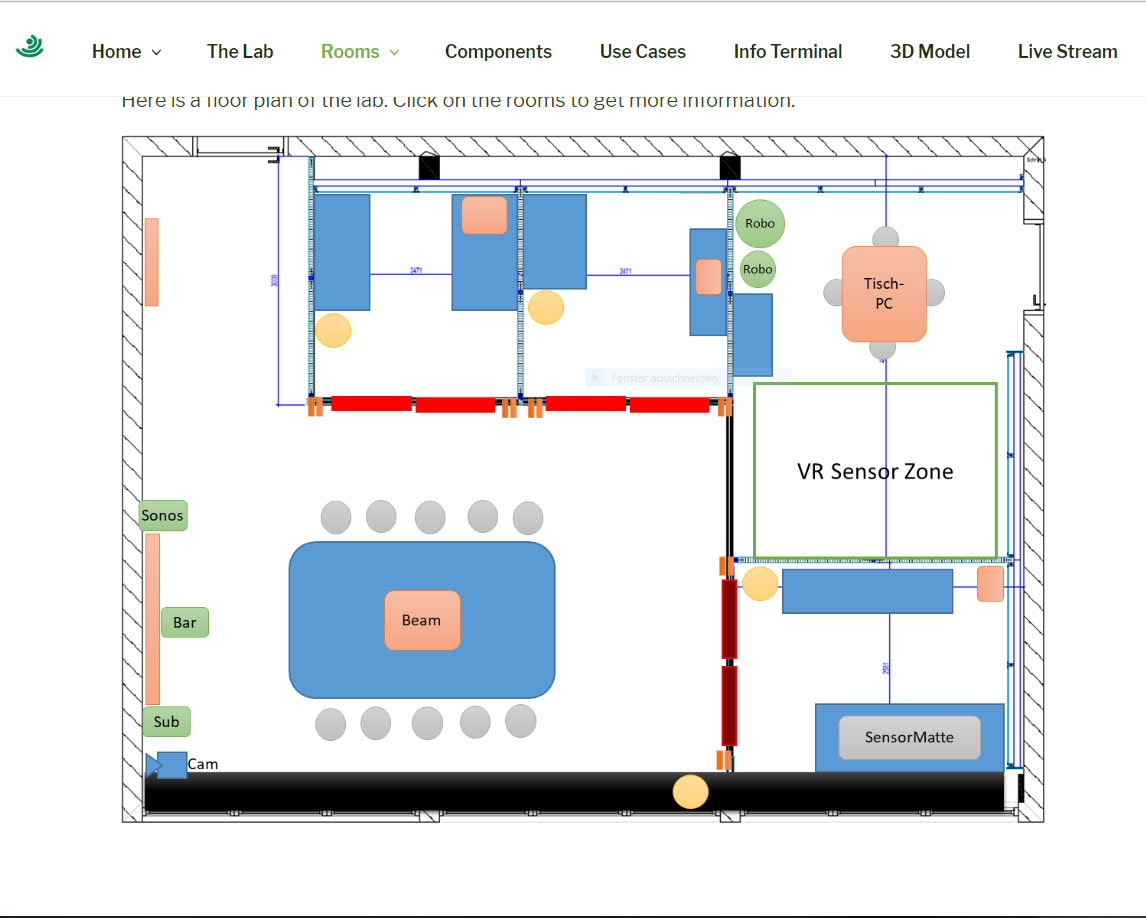
\includegraphics[scale=0.35]{content/pictures/room.jpg}
	% bosch_iot_poll.png: 0x0 pixel, 300dpi, 0.00x0.00 cm, bb=
	\caption{Raumkarte}
	\label{fig:room}
\end{figure}

Jeder Raum hat seine eigene Unterseite, welche die Aufgaben des Raumes und dessen Ausstattung beschreibt.
\newpage
Die Netzwerkarchitektur im Labor ist sehr komplex. Wenn man nicht gerade mit am Aufbau dieser Architektur gearbeitet hat, kann schnell der Überblick verloren werden. Eine Übersichtskarte (siehe Abbildung \ref{fig:network}), auf welcher man sieht wo sich Server, Router und Gateways befinden, kann helfen um herauszufinden, wo bei Problemen mal nachgesehen werden kann. Diese findet man in der Navigation unter dem neuen Punkt Räume. Neben der Karte gibt es zu jedem Raum eine eigene Unterseite, wo auf dessen Netzwerkeigenschaften genauer eingegangen wird. Die Karte wurde mit Adobe Illustrator CC 2017 erzeugt. Dabei wurde, um die Übersichtlichkeit nicht zu gefährden, sehr auf Schlichtheit geachtet. Nur das nötigste wurde eingezeichnet. Neben der Einfachheit halten sich die Farben Grün und Weiß an das \ac{CD} der Hochschule Furtwangen.

\begin{figure}[H]
	\centering
	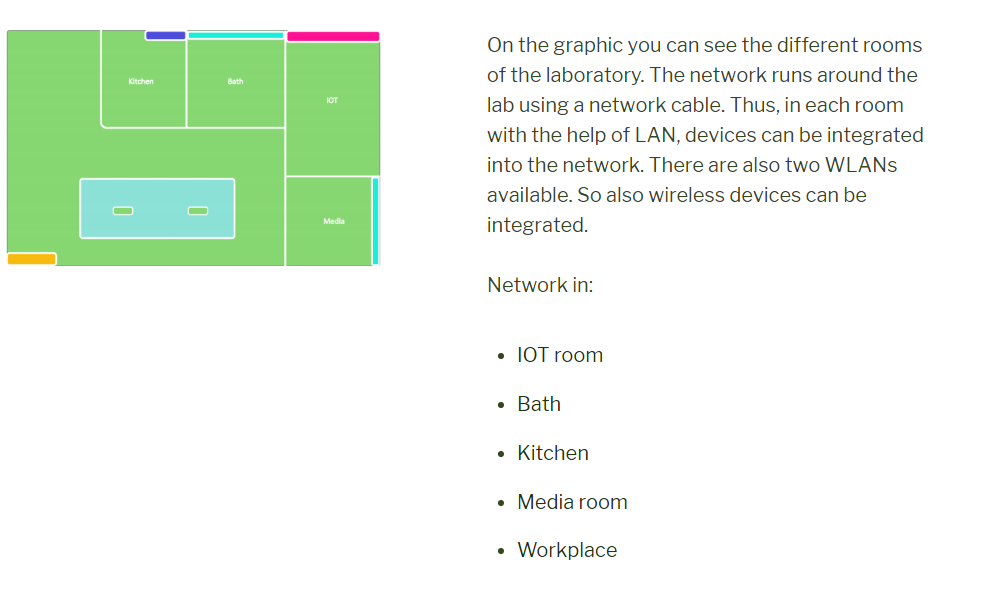
\includegraphics[scale=0.35]{content/pictures/network.png}
	% bosch_iot_poll.png: 0x0 pixel, 300dpi, 0.00x0.00 cm, bb=
	\caption{Netzwerkkarte}
	\label{fig:network}
\end{figure}

\section{Konzeption des Inventarisierungssystem}
\label{konzept:inventar}
Das Inventarisierungssystem ist das Herzstück dieser Masterthesis. Mit ihm können alle Gegenstände verwaltet werden und dazu noch sehr einfach und übersichtlich. Dabei spielt \acf{UX} und damit auch das \acf{UI} eine sehr große Rolle. Um einen Überblick zu bekommen was der aktuelle Markt zu bieten hat, müssen Vergleichbare Verwaltungssysteme(siehe Kapitel \ref{konzept:vergleich}) analysiert werden. Damit eine reibungslose Programmierung erfolgen kann müssen Konzepte für die Architektur der Anwendung ausgearbeitet werden.


\section{Vergleichbare Inventarisierungssysteme}
\label{konzept:vergleich}

Sucht man nach Inventarisierungssysteme stößt man immer wieder auf Software für Webshops. Mit ihnen hat man sehr häufig einen riesigen Umfang an Funktionen, mit welchen man nicht nur sein Inventar, sondern auch seine Verkäufe Verwalten kann.

\subsection{Magento}
\label{konzeption:magento}
Magento\footnote{https://magento.com} ist eine Openen-Source-E-Commerce Plattform und steht unter der Open Software License\footnote{https://opensource.org/licenses/osl-3.0.php}. Umgesetzt wurde es mit dem \acp{PHP} Framework Zend und lässt sich durch zahlreiche Plug-Ins erweitern.\autocite{.2018}

\begin{figure}[H]
	\centering
	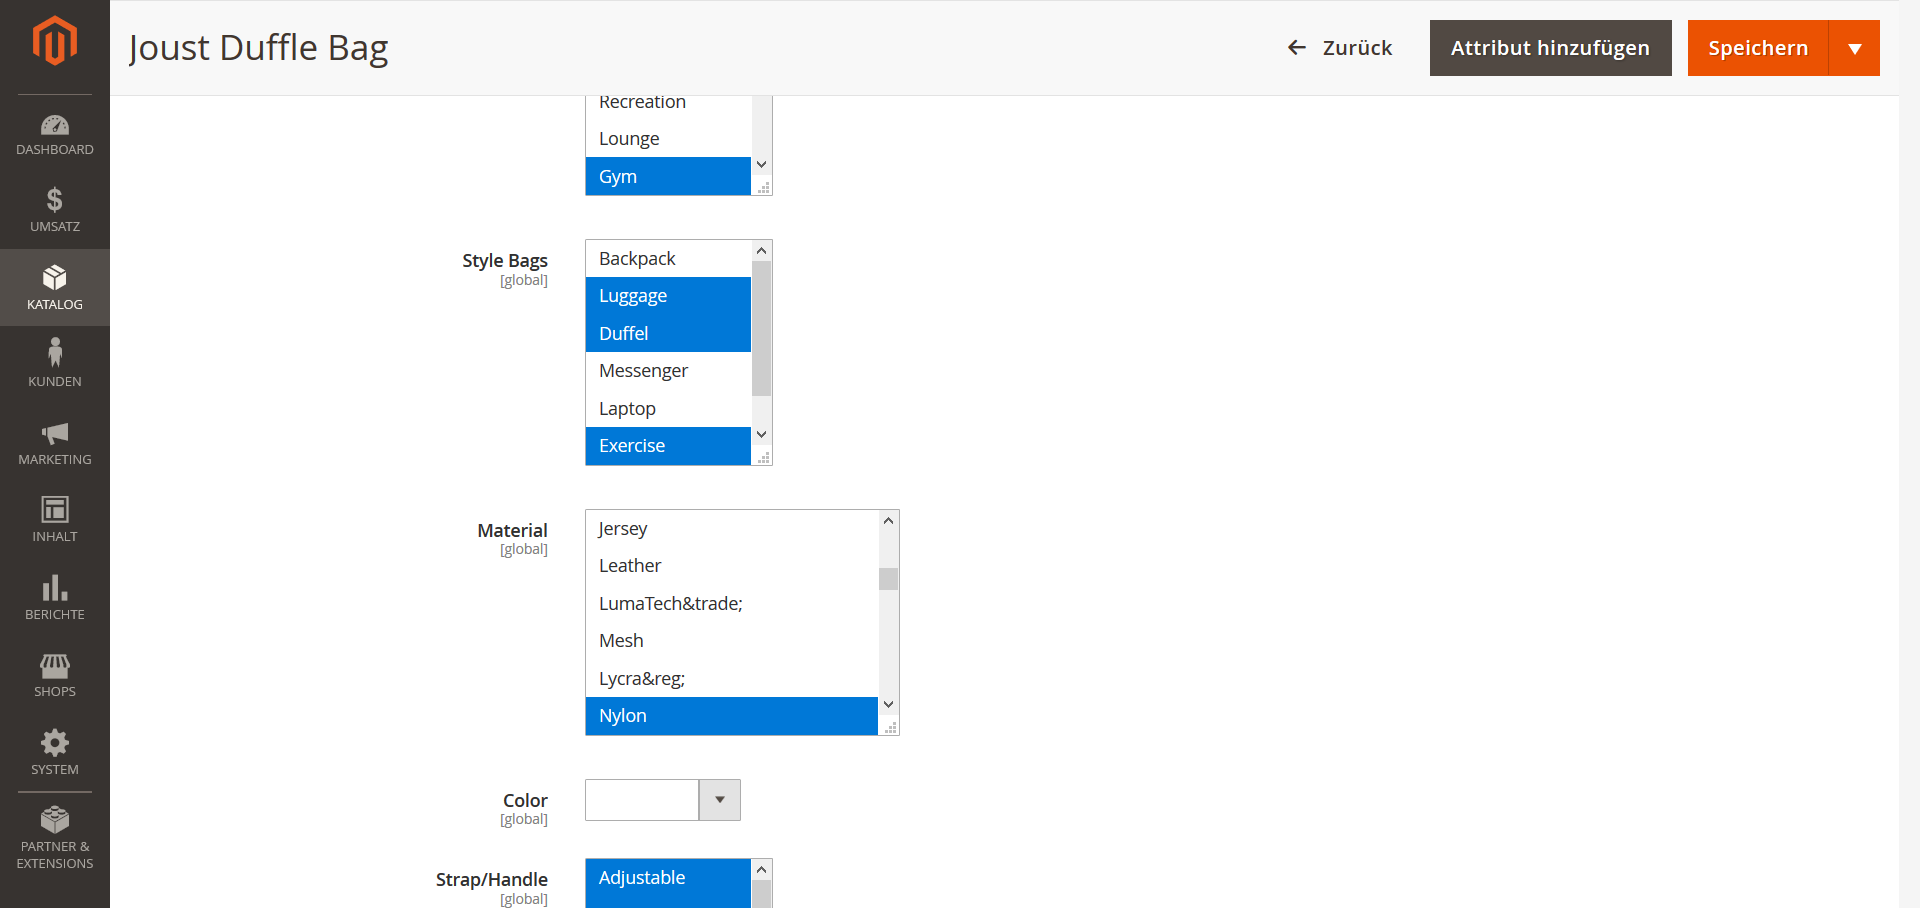
\includegraphics[scale=0.35]{content/pictures/magento.png}
	% bosch_iot_poll.png: 0x0 pixel, 300dpi, 0.00x0.00 cm, bb=
	\caption{Magento Itemverwaltung}
	\label{fig:magento}
\end{figure}

\subsubsection{Vorteile von Magento}
Magento bringt zahlreiche Verwaltungsoptionen. Man kann bis in das kleinste Detail einen Webshop konfigurieren und verwalten. Eine Rollenverteilung der User wird ebenfalls geboten. Jeder Gegenstand kann mit vorgefertigten und eigen angelegten Eigenschaften versehen werden. Das \ac{UI} von Magento ist ähnlich wie bei WordPress sehr benutzerfreundlich. Mit ein wenig Erfahrung findet man sich schnell zurecht. \autocite{Koch.2012}

\subsubsection{Nachteile von Magento}
In seiner größe, liegt der Nachteil des Frameworks. Es bietet zu viele Funktionen, welche nicht für ein Inventursystem in einer Laborumgebung benötigt werden. Damit belegt es unnötig Speicherplatz und lädt Dateien, welche nicht gebraucht werden. Auch wenn die Lernkurve sehr flach ist, muss eine gewisse Einarbeitung doch erfolgen. Auch ist mit der aktuellen Version von Magento eine Aktualisierung der \ac{PHP} Version nötig. \autocite{Koch.2012}

\subsection{WooComerce}
Anders als bei Magento (siehe Kapitel \ref{konzeption:magento}) steht das WordPress-Plugin, welches auch als E-Commerce Software dient unter der \ac{GNU} Lizenz. 

\subsubsection{Vorteile von WooComerce}
Bei Kostenlose WordPress-Plugin ist kostenlos und sehr einfach zu installieren. Mit einem klick ist es aus dem Plugin Bereich gewählt und kann mit einem Installationsassistenten den eigenen Bedürfnissen nach angepasst werden. Ein erfahrener WordPress-Nutzer hat eine deutlich niedrigere Lernkurve, als bei Magento \autocite{WooComerce.2018}

\subsubsection{Nachteile von WooComerce}
Die Nachteile sind ähnlich wie bei Magento. Es beinhaltet zu viele Funktionen, welche nicht gebraucht werden. Außerdem ist es sehr schwer möglich es nicht als Webshop, sondern als Verwaltungssystem zu nutzen. WooComerce gibt hier sehr starke richtlienen vor. So muss man schon im Installationsassisten sich gedanken über Maße, Bezahlmethoden und Versand machen. Was für ein Inventarisierungssystem nicht nötig ist. Mit WComerce ist man stark an WordPress gebunden. Solle man das \ac{CMS} wechseln wollen, ist ein mitnehmen der Anwendung nicht möglich.

\subsection{Entscheidung zur eigenen Anwendung}
Die Entscheidung eine eigene Anwendung zu schreiben wurde schon früh getroffen. Es muss eine Anwendung zur Verfügung gestellt werden, welche nicht mit Funktionen überladen ist. Die Lernkurve muss für jeden Anwender möglichst flach gehalten sein. Der Aufwand Magento oder WooComerce in das Hochschul \ac{CD} zu bringen, kann ein großer Aufwand sein. Daher lohnt es sich die Anwendung selbst zu schreiben. So bleibt sie Konfigurierbar und es werden nur \ac{PHP} Kenntnisse und keine spezielen WordPress oder Magento-Kenntnisse vorausgesetzt. Bei einem Wechsel zu einem anderen \ac{CMS} kann die Anwendung ebenfalls übernommen werden.

\section{Anforderungen}

Mit dem Anforderungsmanagement werden mögliche Features definiert. In der Anforderungsanalyse werden Eigenschaften, Funktionalitäten und die Qualität an die Software Festgehalten. \autocite{Grande.2014} Es werden funktionale und nicht-funktionale Anforderungen niedergeschrieben. Mit diesen Anforderung entsteht eine Definition und Ziele an die Anwendung.

\begin{itemize}
	\item Das Inventarisierungssystem muss alle Items in einer Laborumgebung aufnehmen. 
	
	\item Dabei soll bekannt sein wie der aktuelle Zustand der jeweiligen Items ist. 
	
	\item Die Datenbank sollen durchsuchbar sein. 
	
	\item Es müssen neue Items angelegt und alte gelöscht werden können. 
	
	\item Es soll für jeden Benutzer einen persönlichen Bereich geben. 
	
	\item Es soll Verschiedene Rollen für die Administration und User geben.
	
	\item Jeder Benutzer muss seine Persönlichen Daten verändern können.
	
	\item Benutzer können über den Administrator oder einem dazu befugten Mitarbeiter Items leihen.
	
	\item Benutzer sollen an die Rückgabe der geliehenen Items erinnert werden.
	
	
\end{itemize}

Ist eine solche Liste von Anforderungen erstellt worden, erhält man eine gute Übersicht über die zu entwickelnden Teilbereiche.

\newpage


\section{Datenbank}
\label{konzept:database}

\begin{figure}[bh]
	\centering
	\includegraphics[scale=0.35]{content/pictures/inventarER.png}
	% bosch_iot_poll.png: 0x0 pixel, 300dpi, 0.00x0.00 cm, bb=
	\caption{ER-Diagramm}
	\label{fig:erdiagram}
\end{figure}

Mit der Idee der Webanwendung, wurde schon sehr früh mittels einer Mindmap jede mögliche Eigenschaften aufgeschrieben. Aus dieser Mindmap konnte sehr komfortabel ein ER-Diagramm erzeugt. Um Redundanzen zu vermeiden, muss eine Normalisierung durchgeführt werden. In der Regel sind Redundanzen mit den ersten drei Normalformen abgeschlossen. Im ersten Schritt wurde darauf geachtet, das alle Eigenschaften Atomar sind. Vorname, in der Datenbank firstname und Nachname, in der Datenbank lastname, müssen als einzelne Eigenschaften zur Verfügung stehen. Eine Eigenschaft, mit dem Namen fullname, ist nach der ersten Normalform nicht erlaubt. Um die zweite Normalform zu erfüllen, muss die erste Normalform erfüllt sein und jedes Nichtschlüsselattribut von jedem Schlüsselkandidaten voll funktional abhängig sein. So wird festgestellt welche Eigenschaften eindeutig sind. Das ist nicht immer möglich, wie auch im Fall der Items Tabelle. Jeder Barcode in der Items-Tabelle ist einzigartig, jedoch gibt es Produkte, welche bewusst keinen Barcode haben. Gelöst wurde das Problem mit dem Künstlichen Primärschlüssel ID.\autocite{DatenbankenVerstehen.2018b} Die höchste Priorität der Normalsierung ist das vermeiden von Redundanzen und kann nur mit der 3. Nomalform erreicht werden.  Hierfür wurde die Hilfstabelle Lending eingefügt. Feststellen kann man das, in dem man überprüft, ob es viele-zu-viele existieren. Denn ohne diese Tabelle käme es zu Problemen, wenn sich eine Person mehrere Items leihen möchte.\autocite{DatenbankenVerstehen.2018}


\section{MockUps}
Um die geplante Idee umzusetzen ist es nötig ein MockUp zu erstellen. Doch bevor das MockUp erstellt werden kann, muss Storytelling betrieben werden. Beim Storytelling werden. Beim Storytelling geht es um Geschichten erzählen. Dabei werden die Anforderungen in realistische kleine Geschichten erzählt. So wird es leichter sich vorzustellen, wie ein Programm funktioniert. Diese Geschichten werden sachlich aufgeschrieben. An diesen Geschichten kann früh festgestellt werden, ob sich eine Idee nicht oder nur sehr aufwändig umsetzen lässt. Hier tritt auch die \acl{UX} in den Vordergrund, da man sich beim Schreiben in den User hineinversetzen muss. \autocite{Schach.2017}


\begin{figure}[bh]
	\centering
	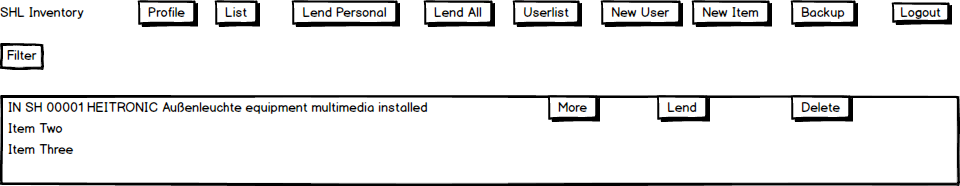
\includegraphics[scale=0.3]{content/pictures/MockUp.png}
	% bosch_iot_poll.png: 0x0 pixel, 300dpi, 0.00x0.00 cm, bb=
	\caption{MockUp von Items-Tabelle}
	\label{fig:mockup}
\end{figure}


Ist das Storytelling abgeschlossen und die möglichen Fehler beseitigt wurden, so kann das MockUp beginnen. Beim MockUp, in der Webentwicklung, wird das Layout schemenhaft mit Bleistift und Papier erzeugt. Dabei tritt das Designe stark in den Hintergrund, es ist in erster Linie wichtig, das verstanden wird, wie die Anwendung mit Button, Formulare und weiteren Elemente funktionieren. Das MockUp macht es später für die Entwicklung leichter, wenn es um die Umsetzung der Webanwendung geht. Bei der Erstellung des MockUp's hat man die Programmierung immer im Hinterkopf. Dabei wird überlegt wie Elemente angelegt werden.

\newpage

\section{User Experience}
\acf{UX} wurde häufiger in dieser Ausarbeitung verwendet und wurde noch nicht genauer erklärt. Das geschieht nun. Bei der \acl{UX}, auf deutsch \textit{Benutzererfahrung}, spricht man davon, wie der Benutzer mit Software Umgeht. Dabei greift man auf eigene Erfahrungen zurück, es gibt allerdings auch Werkzeuge um eine gute Benutzbarkeit zu messen. \autocite{Moser.2012} Dazu gehört Beispielsweise das Storyboard, welches mit hilfe des Storytelling Geschichten mit Bilder erzählt. Für dieses Projekt wurde auf kurze Wege geachtet, das der User die Maus nicht allzu sehr die Maus bewegen. Auch wird dem User durch das Designe gezeigt was klickbar ist und was nicht. Unbewusst wird er eine Gruppierung vornehmen. So sind Buttons, mit welchen etwas erzeugt wird, wie \textit{New Item}, \textit{New User} und \textit{Backup}, mit einem anderen Hintergrund und einer Umrandung versehen. 

\begin{figure}[bh]
	\centering
	
\includegraphics[scale=0.3]{content/pictures/gruppierung.png}
	% bosch_iot_poll.png: 0x0 pixel, 300dpi, 0.00x0.00 cm, bb=
	\caption{Button Gruppierung}
	\label{fig:gruppierung}
\end{figure}

%\subsection{Fitts Gesetze}

\section{Frameworks}
Wenn man Framework in die deutsche Sprache übersetzt, so erhält man das Wort Rahmengerüst. In der Softwareentwicklung spricht man von solchen Frameworks bei Programmierstruckturen, welche den Entwickler unterstützen. Dabei handelt es sich nicht um eine fertige Software. Es handelt sich um bewährte Programmierstruckturen, welche dem Entwickler die Arbeit abnehmen. So werden bekannte Entwurfsmuster übernommen werden. Auch aufwendige Funktionen sind in Frameworks schon häufig implementiert. Der Entwickler muss sich nicht mehr aufwendig um eine Datenverbindung kümmern oder kann komplizierte Animationen mit wenigen Zeilen Code erstellen. Eine wichtige Aufgabe während der Softwareentwicklung ist das Testen. Hier werden mithilfe des Frarmeworks Tests geschrieben, mit welchen kontrolliert werden kann, ob die Software korrekt funktioniert. Frameworks kommen meistens in der Objektorientierung zum Einsatz. Ihre Einsatzgebiete können vielseitig sein. Man findet sie in der Softwareentwicklung, bei der Entwicklung von Spielen und in der Webentwicklung.

\section{Wahl der Frameworks}
\label{chapter:frameworkchoice}
Bei der Wahl der Frameworks wurde analysiert welches sicher läuft, eine große und aktive Community hat, wenig Einrichtungen erfordern und in welchen die meisten Erfahrungen schon vorhanden sind. Bei der Wahl des Frontend-Frameworks fiel die Wahl schon früh auf Angular. Es wird bis heute noch von Google weiterentwickelt und hat eine sehr große Community. Die Erfahrungen in JavaScript sind ebenfalls vorhanden und die meiste Einrichtungen sind schon vorhanden oder werden von dem Framework selbst übernommen. Bei der Wahl des Backend-Frameworks war die Wahl nicht so einfach. Es standen Tomcat, ein Java-Framework und Laravel, ein \acs{PHP}-Framework, zur Auswahl. Es wurde Laravel gewählt, da es von sich aus viele Aufgaben, wie Sicherheit, Datenbankverwaltung oder Benutzerverwaltung mit Login-System übernimmt. \acs{PHP} und MySQL waren auf dem Server installiert. Für Tomcat hätte eine separate Installation erfolgen müssen.

\chapter{Umsetzung}
Mit der Umsetzung des Konzeptes zeigt sich wie gut dieses Gelungen ist. Nachdem nun geklärt ist, wie die Anwendung aussehen soll und welche Werkzeuge verwendet werden, muss eine Testumgebung aufgebaut werden. Ebenfalls muss der Umgang mit den Frameworks und der \ac{IDE}, zu deutsch integrierte Entwicklungsumgebung, vertraut sein.

\section{Aufbau einer Testumgebung}
\label{sec:integration_ace}
Der Server im Smarthome Lab erledigt rund um die Uhr aufgaben. Dabei überwacht er den Zustand verschiedener Geräte und sorgt dafür das diese erreichbar sind. Auf ihm liegen auch Medien und der Webauftritt, welcher über einen Webserver läuft. Dies muss immer zuverlässig funktionieren. Damit der Betrieb nicht eingeschränkt ist, muss eine virtuelle Testumgebung geschaffen werden. Für diesen Zweck wurde ein Abbild des Servers erzeugt, als alles zuverlässig gearbeitet hat. Auf dem Abbild war neben dem Betriebssystem auch der Webserver mit Webauftritt und die MySQL-Datenbank zu finden. Da diese identisch mit den Daten des Servers waren, konnte realistisch getestet werden. Durch das einfache erstellen von Sicherheitskopien konnte risikofrei Software installiert werden um zu schauen, wie sich diese auf das System auswirkt. Mit den verschieden Sicherheitskopien, konnte bei Problemen immer auf einen alten Stand zurückgegriffen werden.


\begin{figure}[bh]
	\centering
	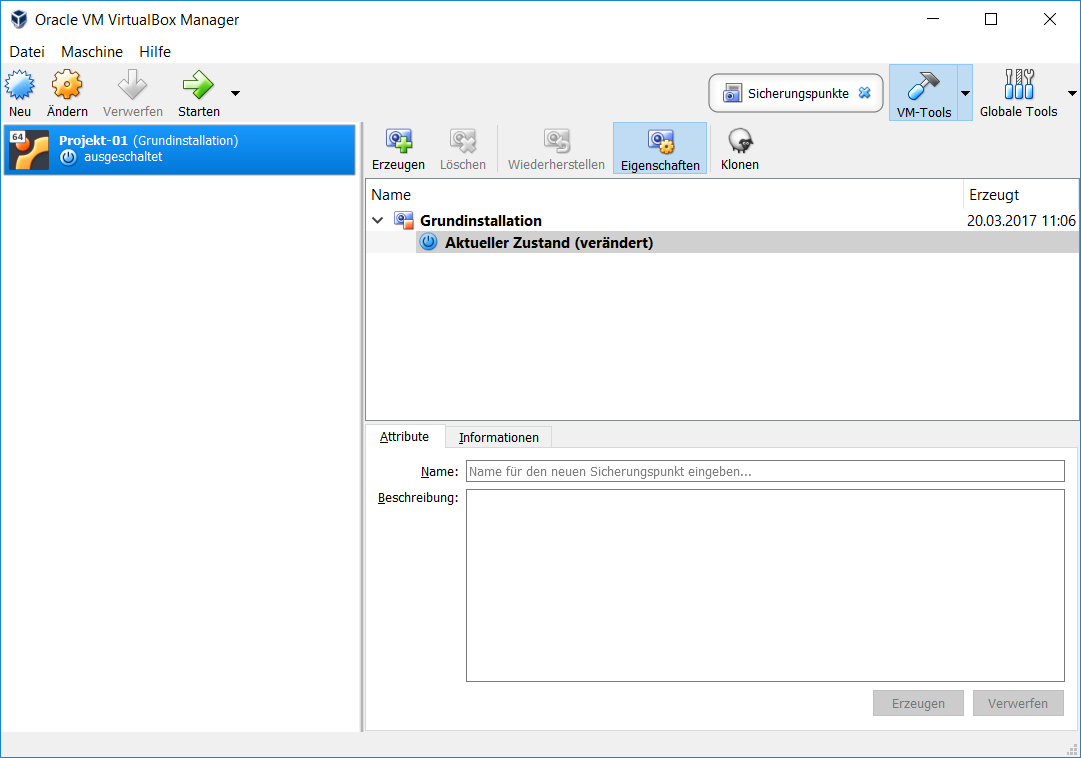
\includegraphics[scale=0.4]{content/pictures/vmware.png}
	% bosch_iot_poll.png: 0x0 pixel, 300dpi, 0.00x0.00 cm, bb=
	\caption{VM-Ware mit geladenem Abbild}
	\label{fig:vmware}
\end{figure}

 In Abbildung \ref{fig:vmware} sieht man den VM-Ware Player. Dieser ist ein kostenloses Tool um Virtuelle Maschinen abzuspielen. Der VM-Ware Player simuliert dabei Hardware, welche im Live-betrieb verändert werden kann. \autocite{vmwareinc.2018} In diesem Fall wird der Server aus dem Smarthome Lab nur Simuliert. Dabei kann ihm mehr speicher hinzugefügt werden, oder auch Seicher entfernt werden. So kam es zu dem Problem, das auf der \ac{VM} nicht ausreichen Festplattenspeicher zur Verfügung stand. In diesem Fall musste die komplette \ac{VM} vergrößert werden. Dies ist mit VM-Ware Player nicht machbar. Unter Windows wird bei der Installation von VM-Ware Player auch der Vdiskmanager installiert. Ein Werkzeug, welches sich über die Kommandozeile steuern lässt. So lässt sich mit dem Befehl \textit{vmware-vdiskmanager -x 100Gb vm.vmdk}, im Verzeichnis der \ac{VM}, die Größe verändern. \autocite{ThomasKrennAG.2018} Damit war ein Vergrößern der \ac{VM} zwar möglich, der zusätzliche Speicher stand zwar physisch, durch eine größere \ac{VM} Datei zur Verfügung, konnte jedoch nicht verwendet werden. In der \ac{VM} wurde ein sogenannter Snapshot verwendet. Bei einem Snapshot, handelt es sich um eine Kopie der \ac{VM} zu einem bestimmten Zeitpunkt. Dieser musste ebenfalls vergrößert werden. Da die Quellen hierzu rar waren, erforderte die Lösung eine lange Suche. Die Lösung ist, mit dem Vdiskmanager den Snapshot auf die gleiche Größe zu bringen. Der Speicher wird nun angezeigt, kann jedoch noch nicht Verwendet werden, da er keiner Partition zugewiesen worden ist. Dies ist über das Betriebssystem, Ubuntu Server 16.04, welches auf der \ac{VM} läuft nicht einfach zu bewerkstelligen. Eine Lösung ist es Ubuntu 18.04 zu verwenden. Dabei wir ein Abbild der DVD, welche für die Installation von Ubuntu benötig wird, in das Virtuelle DVD Laufwerk gelegt. Ubuntu kann ohne Installation verwendet werden. Es liefert das Programm GPartet, mit welchem sich der neue, noch nicht zugewiesene Speicher, der Serverpartition zuweisen lässt. Mit einem Neustart der \ac{VM} und dem Entfernen des Images aus dem virtuellen Laufwerk, hat die \ac{VM} nun ausreichend Festplattenkapazität.\autocite{automatix.}

\subsection{Integration in das Netzwerk}
Da es sich bei der \ac{VM} um ein direktes Abbild des Servers im Smarthome Lab ist, hat es auch die identischen Eigenschaften. So auch die. 

\subsection{MySQL}
Passwort nicht zur verfügung. Neuinstallation notwendig.

\subsection{Nginx}

\section{XAMPP}
Nur für PHP und MySQL lokal 

\section{Austausch von Daten}




\section{Frontend}

\subsection{Commandlineinterface}

\subsection{TypeScript}
Objektorientiert

\subsection{Module}
HTTP

\subsection{Components}

\subsection{Services}





\section{Backend}

\subsection{Composer}

\subsection{Controller}

\subsection{REST}

\subsection{Webserver}


\section{Security}

\subsection{CORS}

\subsection{Token}

\subsection{Salt}


\section{Deploy}

\chapter{Anwendung}
Dieses Kapitel soll die Interessantesten Teile der Anwendung Dokumentieren. Mit dem Vorangegangen Code lassen sich alle nicht dokumentierte Teile im Code sehr gut nachvollziehen.



\section{Anlegen, Aktualisieren, Löschen und Ausgeben von Gegenständen}
Im Frontend werden neue Gegenstände über ein Formular gesendet. Die Inhalte des Formulars werden per \ac{JSON} mittels POST an die Restschnittstelle von Laravel gesendet, welche der Controller verarbeitet und in die Datenbank einträgt. Sollte ein Barcode schon vorhanden sein, wird der User darauf hingewiesen. Bei einer Löschung, Aktualisierung oder einer Ausgabe muss nur darauf hingewiesen werden, um welches Item es sich genau handelt.

\begin{lstlisting}[language=php, frame=single]
public function postItem(Request $request)
{
$item = new Item();
$item->barcode = $request->input('barcode');
$item->name = $request->input('name');
$item->description = $request->input('description');
$item->type = $request->input('type');
$item->room = $request->input('room');
$item->status = $request->input('status');
$item->annotation = $request->input('annotation');
$item->image = $request->input('image');
$item->lend = $request->input('lend');
$item->manufactor = $request->input('manufactor');
$item->save();
return response()->json($item, 201);

}

public function getItems(){
$items = Item::all();
$response = [
'items' => $items
];
return response()->json($response,200);
}

public function putItem(Request $request, $id){
$item = Item::find($id);
if(!$item){
return response()->json(['message'=>'Document not found Barcode: '. $id . '. The number is not the Barcode. Look into the Table'], 400);

}
$item->name = $request->input('name');
$item->description = $request->input('description');
$item->type = $request->input('type');
$item->room = $request->input('room');
$item->status = $request->input('status');
$item->annotation = $request->input('annotation');
$item->image = $request->input('image');
$item->lend = $request->input('lend');
$item->manufactor = $request->input('manufactor');
$item->save();
return response()->json(['item' => $item], 200);
}

public function putItemLendBack( $id){
$item = Item::find($id);
if(!$item){
return response()->json(['message'=>'Document not found putItemLendBack: '. $id . '. The number is not the Barcode. Look into the Table'], 400);

}

$item->status = 'back';

$item->save();
return response()->json(['item' => $item], 200);
}

public function deleteItem($id){
$item = Item::find($id);
$item->delete();
return response()->json(['message' => 'Deleted'],200);

}

public function getItem($id){
$item = Item::find($id);
if(!$item){
return response()->json(['message'=>'Document not found ID: '. $id . '. The number is not the Barcode. Look into the Table'], 400);

}

$response = [
'items' => $item
];

return response()->json($response,200);


}
\end{lstlisting}

\begin{figure}[H]
	\centering
	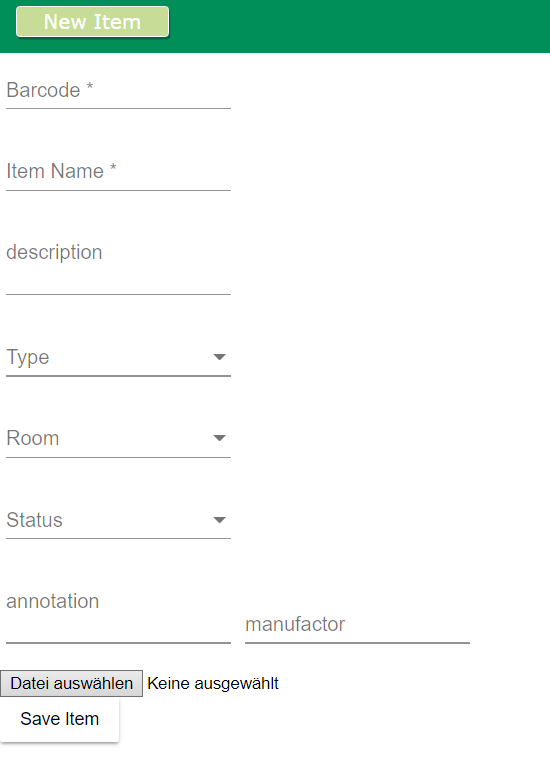
\includegraphics[scale=0.5]{content/pictures/item.png}
	% bosch_iot_poll.png: 0x0 pixel, 300dpi, 0.00x0.00 cm, bb=
	\caption{Anlegen von Items}
	\label{fig:item}
\end{figure}

\section{Ausgabe von allen Gegenständen}
Um eine Liste aller Gegenstände wird vom Server eine \ac{JSON} generiert, welche mit in Angular in einer Tabelle ausgegeben werden. Hierfür wurde Angular Material verwendet, welches die Tabelle auch gleichzeitig gestaltet hat.

\begin{lstlisting}[language=html, frame=single]
<mat-table [dataSource]='dataSource' matSort>

<ng-container matColumnDef="barcode">
<mat-header-cell *matHeaderCellDef mat-sort-header>Barcode</mat-header-cell>
<mat-cell *matCellDef="let items">{{items.barcode}}</mat-cell>
</ng-container>

.
.
.

<mat-header-row *matHeaderRowDef="displayedColumns"></mat-header-row>
<mat-row *matRowDef="let row; columns: displayedColumns;"></mat-row>

</mat-table>
\end{lstlisting}


\section{Routing Strategie}
Wie in Kapitel \ref{webauftritt} beschrieben, wird der Webauftritt von WordPress verwaltet. WordPress selbst nutzt das Routing um Verschiedene Seiten anzeigen zu können. Läuft eine Angular Anwendung auf dem gleichen Server, oder soll sie gar in WordPress eingebunden werden, kann das zu Problemen führen, da sie die gleiche Strategie nutzen. Eine Unterseite in Angular aufzurufen ist nicht möglich wenn man es zuvor nicht konfiguriert. WordPress wird immer eine Fehlerseite werfen, sofern nicht eine Unterseite von WordPress den gleichen Namen trägt. Aber auch in diesem Fall wird eine Falsche Seite dem User Präsentiert.

Eine Lösung ist die \textit{HashLocationStrategy}. Bei dieser Strategie muss der Anwendung mit einem Konfigurationsbefehl mitgeteilt werden, wie das Routing ab sofort funktionieren soll. Dabei wird vor der dem eigentlich Anhängen der Unterseite ein Rautensymbol angehangen. Damit kann Wordpress in der Regel nur die Startseite Anzeigen und wird nicht auf eine Fehlerhafte Seite verweisen. Somit ist ein Routing unter der gleichen Domain möglich und es ist trotz allem für den User nachvollziehbar. 

\begin{lstlisting}[language=sh, frame=single]
RouterModule.forRoot(routes, {useHash: true})
\end{lstlisting}

Es ist nur useHash im Routermodul auf true zusetzen und Angular erledigt den rest. Die variable routes ist ein Array, welches alle Routen verwaltet.



\section{E-Mail Reminder}
Für den Reminder (\ac{z. Dt.} Erinnerer) wird eine Konfiguration angelegt, in welcher definiert wird was in der E-Mail stehen soll, welche der User erhalten wird. Dabei handelt es sich um ein Template. Alle nötigen Daten holt sich Laravel selbständig aus der Datenbank. Ein Anlegen eines solchen Schedulars wird im folgenden Code Beispiel Demonstriert.
\begin{lstlisting}[language=php, frame=single]
protected function schedule(Schedule $schedule)
{
		$schedule->command('reminder:mail')->daily();
}
\end{lstlisting}

\section{Datenbank import und export}
Für einen unerfahrenen User soll es leicht sein Daten zu importieren und für eine Sicherung oder zur Nutzung ohne Netzwerkverbindung zu nutzen. Auch kann es sein, das viele Daten Angelegt werden sollen, welche einfacher oder schneller über eine Tabelle angelegt werden könnten. Dabei soll der User keine Daten anlegen oder mit Programmen arbeiten müssen, welche ihm unbekannt sind. Eine sehr Bekannte Möglichkeit solche Dateien zu erstellen ist Microsoft Excel. Der User soll eine Excel-Datei erstellen und diese über ein grafische Benutzeroberfläche importieren können. Dabei darf es keine Rolle spielen welche Endung die Excel-Datei hat. Mit einem Export soll ebenfalls eine Excel-Datei erzeugt werden.

Für den Import wurde mittels Composer die Erweiterung PHPOffice verwendet. Es kann Excel-Dateien lesen und schreiben. Mit dem Lesen werden die Daten in die Datenbank geschrieben. Hierbei wird Dopplung vermieden und wenn es sich um bekannte deutsche Begriffe handelt, werden diese auf englisch in die Datenbank geschrieben. Sollte ein Begriff unbekannt sein, so wird der deutsche Wortlaut übernommen. Um Dopplung zu vermeiden musste ein eindeutiger Schlüssel gewählt werden. Die Entscheidung fiel auf den Barcode. Hat ein neu angelegtes Item keinen Barcode, wird es nicht importiert. Dieser ist zwingend nötig. Der Export wird ebenfalls von PHPOffice übernommen. Hierbei muss nur Angegeben werden, wie jede Spalte heißt. Der User kann nun sich einmalig eine Tabelle Exportieren lassen und diese nach diesem Schema füllen und Importieren. Die Exportieren Funktion findet der User Unter dem Button Backup.

\begin{lstlisting}[language=php, frame=single]
public function insertItemsInDatabase()
{
	$inputFileName = public_path() . '\table\barcode.xlsx';
	$inputFileType = IOFactory::identify($inputFileName);
	
	$reader = new \PhpOffice\PhpSpreadsheet\Reader\Xlsx();
	
	
	$reader->setReadFilter(new MyReadFilter());
	
	//Einlesen
	$spreadsheet = $reader->load($inputFileName);
	
	$sheetData = $spreadsheet->getActiveSheet()->toArray(null, true, true, true);
	
	
	//alle datein eintragen und übersetzen
	foreach ($sheetData as $row){
		
		$name ="";
		$barcode ="";
		$description ="";
		$room ="";
		$status ="";
		$type ="";
		$annotation ="";
		$image ="";
		$lend ="";
		$manufactor ="";
		
		
		
		//Übersetzung
		if($row['F'] == 'Zubehör'){
			$type = 'equipment';
		}
	
	...	
		
		//Abbruchkreterium
		if (DB::table('items')->where('barcode', '=', $barcode)->count() > 0) {
			continue;
			
		}
		else{
			DB::table('items')->insert(
			['barcode'=> $barcode, 'name' => $name, 'description' => $description,
			'type' => $type, 'room' => $room, 'status' => $status]
			);
		}
			
		
	}
	
	return response()->json($sheetData, 200);
	
}
\end{lstlisting}

\begin{lstlisting}[language=php, frame=single]
 public function exportItemsInXml(){
//Überschriften für die Spalten
$spreadsheet = new Spreadsheet();
$sheet = $spreadsheet->getActiveSheet();
$sheet->setCellValue('A1', 'Artikel');
$sheet->setCellValue('B1', 'Barcode');
$sheet->setCellValue('C1', 'Bezeichnung');
$sheet->setCellValue('C1', 'Bezeichnung');
$sheet->setCellValue('D1', 'Einsatzbereich');
$sheet->setCellValue('E1', 'Position');
$sheet->setCellValue('F1', 'Kategorie');
$sheet->setCellValue('G1', 'Status');

$items = Item::all();

$exportFileName = "table\\barcode_export.xlsx";

//Eintragen der Daten
foreach ($items as $item){
$sheet->setCellValue('A' . $index, $item->name);
$sheet->setCellValue('B'  . $index, $item->barcode);
$sheet->setCellValue('C' . $index, $item->description);

$sheet->setCellValue('D' . $index, $item->room);
$sheet->setCellValue('E' . $index, 'unknown');
$sheet->setCellValue('F' . $index, $item->type);
$sheet->setCellValue('G' . $index, $item->status);
$index++;
}

$writer = new Xlsx($spreadsheet);



$writer->save($exportFileName);



//in eine Datei schreiben.
return response()->download(public_path('table\\barcode_export.xlsx'))->deleteFileAfterSend();

}
\end{lstlisting}

\begin{figure}[H]
	\centering
	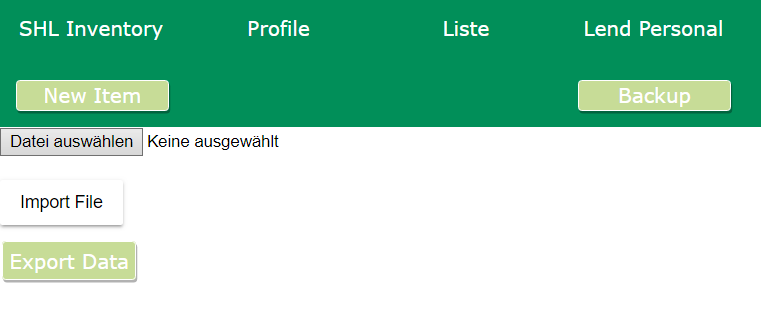
\includegraphics[scale=0.5]{content/pictures/backup.png}
	% bosch_iot_poll.png: 0x0 pixel, 300dpi, 0.00x0.00 cm, bb=
	\caption{ Importieren und Exportieren von Items}
	\label{fig:backup}
\end{figure}

\section{Gestalten der Navigationsleiste}
Die Webanwendung ist nicht responsiv. Was heiß das sich nicht auf allen Endgeräten perfekt dargestellt und nur auf einem PC oder Tablett komfortabel genutzt werden kann. Jedoch wurde mittels \ac{CSS}3 eine Navigation gestaltet, welche sich der Größe des Browsers anpasst.


\begin{lstlisting}[language=php, frame=single]
.felx-container {
	display: flex;
	background-color: #018F59;
	width: 100%;
	margin-left: auto;
	margin-right: auto;
	flex-direction: row;
	flex-wrap: wrap;
	justify-content: space-between;
	
	span {
		color: white;
		margin: .8rem;
		width: 120px;
		text-align: center;
		
		
	}
	
}

\end{lstlisting}
\chapter{Diskussion der Ergebnisse}
\label{cha:discussion}
Die Arbeit verlief zu großen Teilen sehr gut. Auf einem lokalen System läuft Sie reibungslos und erfüllt ihre Aufgaben. Dies ist auf dem Server nicht der Fall. Das Deploy ist gescheitert und somit auch die Implementierung. Sollte ein Deploy noch nachträglich umgesetzt werden, so handelt es sich hierbei um ein funktionierende Inventursystem für das Smarthomelab der Hochschule Furtwangen.



\section{Fazit}
Für mich ist das Projekt ein Erfolg. Es hat mich in meinem Wissen weitergebracht und ich habe eine Anwendung umgesetzt, welche alle Phasen durchlaufen ist. Schade ist es, das es am Ende an dem Deploy gescheitert ist. Aber aus diesen Fehlern habe ich gelernt. Ich hätte mit einem Zwischenergebnis die Tücken eines Deploys feststellen können und wäre darauf besser Vorbereitet. Auch wenn die Konzeptionszeit sehr gut verlief, würde ich diese in einem zweiten Anlauf verkürzen. Nichts desto weniger bin ich sehr zufrieden mit dem Ergebnis.


\section{Ausblick}
Auf dieser Arbeit lässt sich aufbauen. So wurde eine \ac{REST}-Schnittstelle entwickelt. Hier könnte man Ansetzen und einen Barcodescanner entwickeln welcher auf diese Schnittstelle zugreift. Dabei spielt es noch nicht einmal eine Rolle um welche Programmiersprache es geht, solange sie REST-Befehle senden kann. Auch könnte mit einer Schnittstelle zu OpenHAB die Status der einzelnen Items erweitert werden. So das man in der Tabelle schon sehen kann welches Item in Betrieb ist. Als Beispiel könnte man zeigen, welche Lampen in welcher Farbe leuchten.



% Schalgwortverzeichnis (Index)
%\printindex

% Literaturverzeichnis


\singlespacing
%\bibliographystyle{alphadin}
%\bibliography{bibitems}
%\addbibresource{bibitems.bib}
\printbibliography

% Eidesstattliche Erklärung
\chapter*{Eidesstattliche Erklärung\markboth{Eidesstattliche Erklärung}{}}
% Eintrag in das Inhaltsverzeichnis 
\addcontentsline{toc}{chapter}{Eidesstattliche Erklärung}

Ich versichere, dass ich die vorstehende Arbeit selbständig verfasst und hierzu
keine anderen als die angegebenen Hilfsmittel verwendet habe. Alle Stellen der Arbeit die 
wörtlich oder sinngemäß aus fremden Quellen entnommen wurden, sind als solche kenntlich gemacht.\\\\
Die Arbeit wurde bisher in gleicher oder ähnlicher Form in keinem anderen
Studiengang als Prüfungsleistung vorgelegt oder an anderer Stelle
veröffentlicht.\\\\
Ich bin mir bewusst, dass eine falsche Erklärung rechtliche Folgen haben kann.

\vspace*{1.5cm} \par
\line(1,0){200} \par
\docOrt, den  \docAbgabedatum ~~\docVorname~\docNachname

%\appendix
% Hier können Anhaenge angefuegt werden
%\chapter{Anhang}
CD mit dem Gesamten Code und der LaTex-Dateien
  
\end{document}      
